La base informativa è incentrata sui dati più importanti per la nostra applicazione, ovvero esercizi, classi e utenti. Ogni esercizio salvato nel database ha, inoltre, una o più soluzioni.

\begin{itemize}
	\item \texttt{Exercise}: ogni esercizio viene identificato da un codice e possiede una frase (univoca all'interno del database);
	\item \texttt{Class}: ogni classe viene identificato da un codice, possiede un nome (univoco) e dei riferimenti agli studenti, all'insegnante e agli esercizi ad esso assegnati;
	\item \texttt{User}: ogni utente viene identificata da un codice, possiede dei dati personali (come nome, cognome, città, scuola) e le credenziali di accesso; inoltre, se l'utente non è un insegnante il campo \texttt{teacher} contiene \texttt{-1}.
\end{itemize}

\begin{figure}[ht]
	\centering
	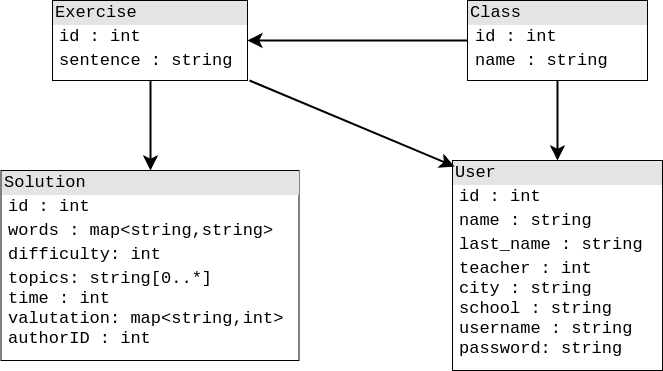
\includegraphics[scale=0.65]{images/database.png}
	\caption{Schema della base informativa}
\end{figure}